\begin{figure*}[!htb]
    \begin{subfigure}{\linewidth}
        \caption{}
        \centering
        % include first image
        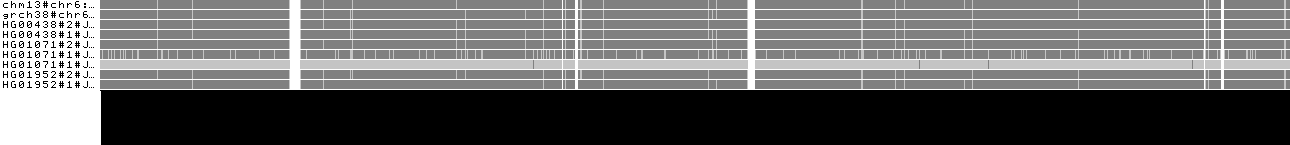
\includegraphics[width=1.0\linewidth, trim=-0cm 0cm 0 0cm]{fig/sorting/chr6_pan_fa_a2fb268_4030258_6a1ecc2_smooth_mhc_random_sorted}
        \label{fig:mhc-random-node-order}
        \vspace{-2em}
    \end{subfigure}
    \begin{subfigure}{\linewidth}
        \caption{}
        \centering
        % include first image
        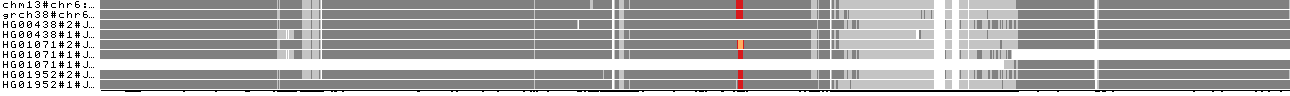
\includegraphics[width=1.0\linewidth, trim=-0cm 0cm 0 0cm]{fig/sorting/chr6_pan_fa_a2fb268_4030258_6a1ecc2_smooth_mhc_PGSGD_sorted}
        \label{fig:mhc-pgsdg-sorting}
        \vspace{-2em}
    \end{subfigure}
    \begin{subfigure}{1\linewidth}
        \caption{}
        \centering
        % include fourth image
        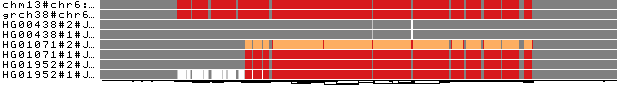
\includegraphics[width=1.0\linewidth, trim=-0cm 0.5cm 0 0cm]{fig/sorting/chr6_pan_fa_a2fb268_4030258_6a1ecc2_smooth_C4_PGSGD_sorted}
        \label{fig:c4-pgsdg-sorting}
    \end{subfigure}
    \begin{subfigure}{1\linewidth}
        \caption{}
        \centering
        % include fourth image
        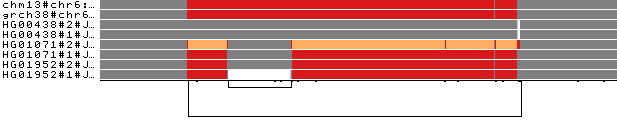
\includegraphics[width=1.0\linewidth, trim=-0cm 0.5cm 0 0cm]{fig/sorting/chr6_pan_fa_a2fb268_4030258_6a1ecc2_smooth_C4_topologically_sorted}
        \label{fig:c4-topological-sorting}
    \end{subfigure}
    \caption{
        Sorting and visualizing the human major histocompatibility complex (MHC) and complement component 4 (C4) pangenome graphs.
        All visualization are made with \textit{odgi viz} by coloring the paths by node depth:
        using the Spectra color palette with 4 levels of node depths, white indicates no depth, while grey, red, and yellow indicate depth 1, 2, and greater than or equal to 3, respectively.
        \textbf{(a)} Visualization of a MHC pangenome graph with nodes randomly sorted from left to right.
        The image shows a region 5 Mbp-long.
        The bad node order completely hides the linear graph structure.
        \textbf{(b)} Visualization of the same MHC pangenome graph but sorted by applying the path-guided stochastic gradient descent algorithm (PG-SGD).
        The graph globally shows a linear structure, without long range links (at the bottom of the image).
        Furthermore, the C4 region is visible as a region with red and orange paths.
        \textbf{(c)} Visualization of the PG-SGD sorted C4 subgraph.
        The image shows a region 83361 bp-long.
        The C4 region is still not well sorted locally, with the node order that still hides the underlying copy number variation status present in such a region.
        \textbf{(d)} Visualization of the same C4 pangenome graph but sorted by applying a topological sorting.
        The graph shows its structure: the two references present two different allele copies of the C4 genes (in red), both of them including the HERV sequence.
        HG01071\#2 presents 3 copies of the \textit{locus} (orange), of which one contains the HERV sequence (gray in the middle of the orange).
        In HG01952\#1, the HERV sequence is absent (white in the middle of the red).
    }
    \label{fig:sorting}
\end{figure*}
